\newpage
\noindent
\vspace*{-2.0cm}
\section*{\sectionformat Arroz Grudado}
\addcontentsline{toc}{section}{Arroz Grudado}
\vspace*{-0.1cm}
\begin{aemulticol}[width=0.495\textwidth,height=0.545\textheight]
	\begin{tabu} to 0.5\linewidth {X[l]X[r]}
	   \textit{Serve 4 pessoas} & \textit{300 kcal}
	\end{tabu}\\
	\rule[0.5ex]{0.5\linewidth}{1pt}	
	\vspace*{-0.3cm}
	\subsection*{\subsectionformat Ingredientes}
	\vspace*{-0.15cm}
	\begin{tabu} to 0.5\linewidth {X[l]X[l]}
	   $\bullet$ uma caneca de arroz & $\bullet$ um quarto de cebola\\$\bullet$ três dentes de alho & $\bullet$ uma colher de sopa de azeite\\$\bullet$ sal a gosto & $\bullet$ duas canecas e meia de água

	\end{tabu}
	\vspace*{-0.15cm}
	\subsection*{\subsectionformat Modo de Preparo}
	\vspace*{-0.15cm}
	1. Colocar a água para ferver em uma panela.\\
2. Picar a cebola e o alho em pequenos cubos.\\
3. Colocar o azeite em uma panela e aquecer.\\
4. Refogar inicialmente a cebola e em seguida adicionar o alho.\\
5. Adicionar o arroz e mexer bem. Cuidado para não queimar.\\
6. Adicionar a água fervente à mistura e mexer um pouco.\\
7. Acrescentar o sal e mexer um pouco.\\
8. Manter fogo médio para alto até a água atingir o nível do arroz.\\
9. Deixar a panela meio fechada e o fogo de baixo para médio.\\
10. Checar com um garfo o nível da água.\\
11. O arroz estará pronto quanto houver muito pouca ou nenhuma água restante no fundo da panela.

	\vspace*{-0.15cm}
	\subsection*{\subsectionformat Dicas}
	\vspace*{-0.15cm}
	$\bullet$ Enquanto estiver esperando a água atingir o nível do arroz, prove-a com uma colher para ajustar o nível de sal caso seja necessário.

	\vspace*{-0.15cm}
	\subsection*{\subsectionformat História}
	\vspace*{-0.15cm}
	\textit{Após anos de arroz grudento, resolvemos descobrir como se faz arroz solto.}
\end{aemulticol}
\begin{tikzpicture}[remember picture, overlay]
\node[anchor = south, inner sep = 0pt, outer sep = 0pt] at (current page.south){
	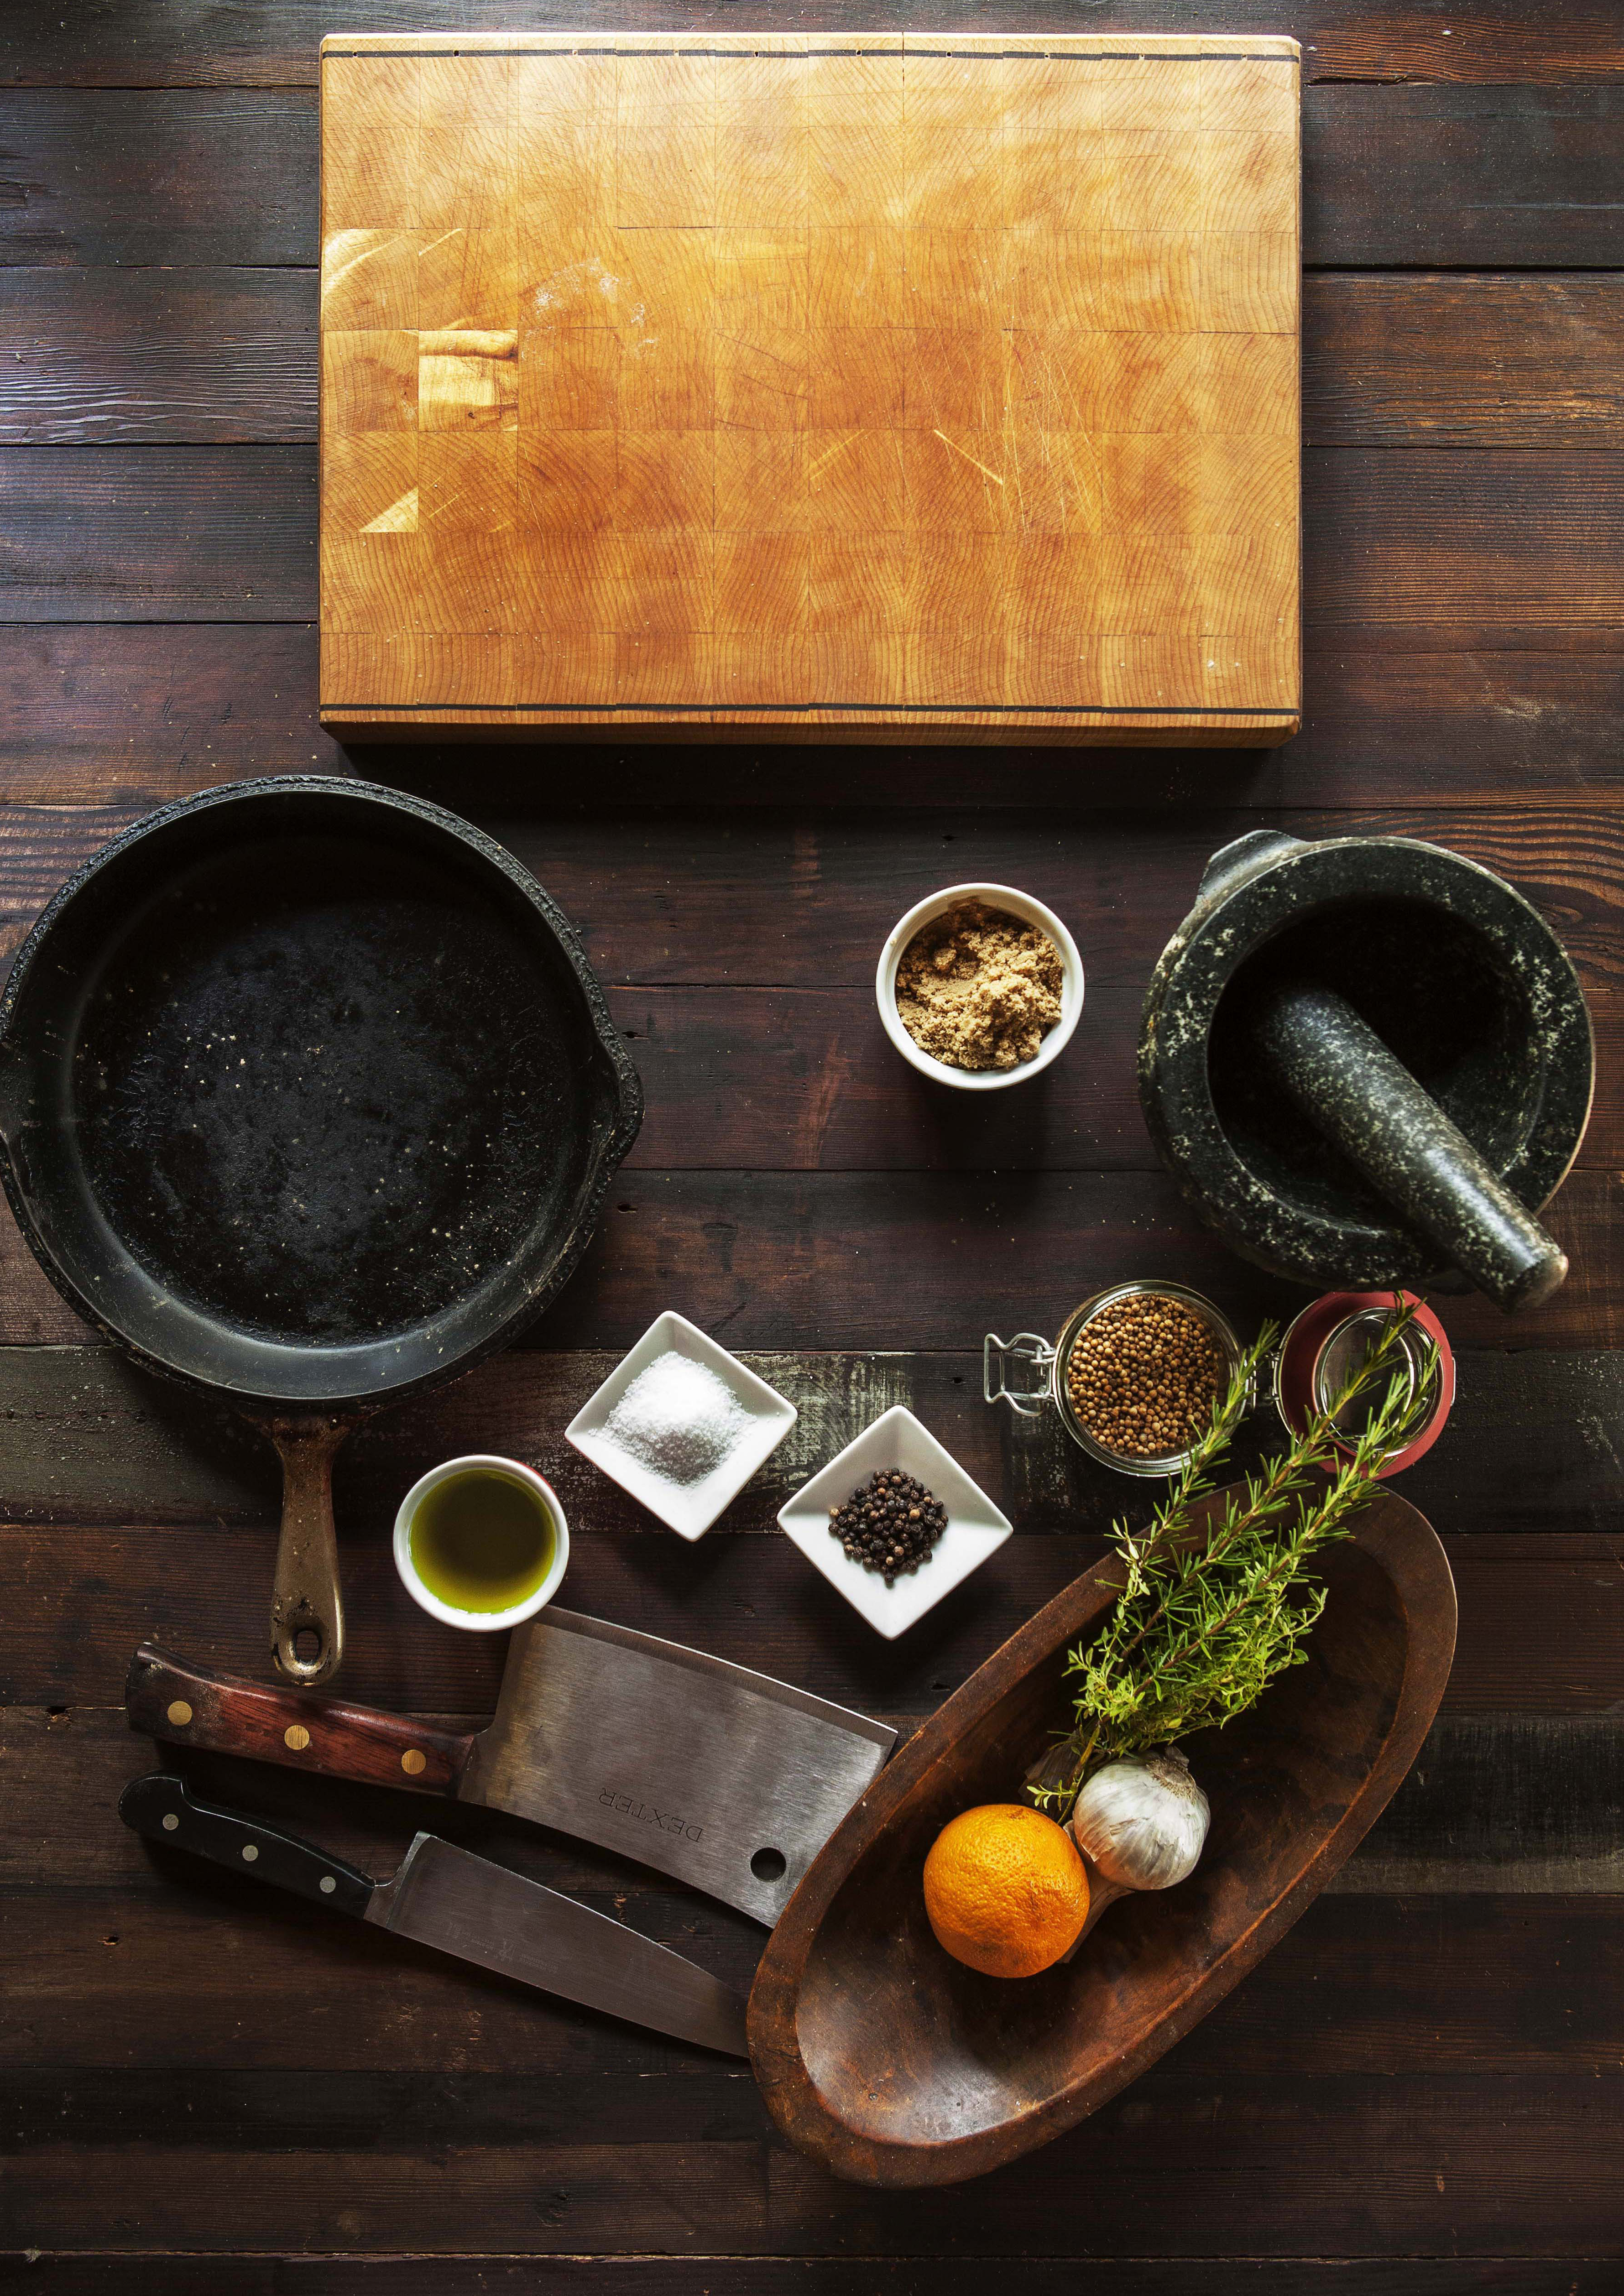
\includegraphics[width=\paperwidth, height=0.45\paperheight]{cover.jpg}
};
\end{tikzpicture}
